

\chapter{Konzeptionierung einer integrierten Python Anwendung}\label{PythonApp}

Die Basisanforderungen einer integrierten LZ-Verwaltung lassen sich aus Kapitel \ref{Kap2} ableiten.
Hinzu kommen die später in Kapitel 5 beschriebenen Funktionen.
Anhand dieser beiden Punkte kann man erkennen, dass Modularität, Erweiterbarkeit sowie Wartbarkeit wichtige Kriterien sind.
Darüber hinaus müssen diese Schritte auch von Personen durchgeführt werden können, die mit der ursprünglichen Entwicklung
der Software nicht involviert waren.
Eine saubere Struktur der Software ist dazu unerlässlich.
Die alte Software nutzte eine GUI-Klasse als Datenhub.
Dadurch entstand ein unübersichtliches Klassenkonstrukt, sodass es für Außenstehende sehr schwer wurde sich in den Code
einzudenken.
Dadurch, dass Teile der Programmlogik in den XAML Dateien \glqq versteckt\grqq wurden, wurde es beinahe unmöglich.
Zum Beispiel wird anhand der Klassendiagramme deutlich, dass Daten der Modbus Adressen in die \verb|commissionMatrix|
geschrieben werden müssen, weil ausschließlich dort zu RAPID Kommandos übersetzt werden und an den ABBRobotics Controller
übergeben werden.
Wie genau das passiert, lässt sich anhand des C\# Codes nicht nachvollziehen.
Ich bin mir sicher, dass mit einer Menge Zeitaufwand dieses Rätsel gelöst werden kann, jedoch bringt es für die
Konzeptionierung der neuen Software keinen Mehrwert.\\
\vspace{1cm}
Um diese Unannehmlichkeiten für die Zukunft zu vermeiden, empfiehlt es sich auf branchenübliche Design Patterns zurückzugreifen.
Das grundlegendste Design Konzept ist das MVC.
Dieses Konzept sieht vor, dass Daten (Model) und GUI (View) keinerlei Zugriff aufeinander erlauben.
Die Schnittstelle zwischen den Daten und dem Benutzer ist ein Controller, der die Programmlogik implementiert.
Für die Daten gilt, dass sie in einer Objektstruktur modelliert werden und nicht von außerhalb dieser Objekte verändert
werden.
\vspace{1cm}
Soll ein Wert in dem Datenmodell geschrieben oder verändert werden, dann muss dafür eine öffentliche Methode existieren,
die alle möglichen Fehler abfängt und referenzielle Integrität herstellt. \\
Als Beispiel für die referenzielle Integrität möchte ich eine Palette mit einem Becher anführen.
In Abb. \ref{fig:figure9} sind drei Klassen, Pallet, Cup und Product, dargestellt.
Die Attribute der Klassen sind private, was durch das \glqq - \grqq angedeutet ist.
Ein Objekt der Klasse \verb|Pallet| kann sich also nicht direkt selbst in das entsprechende Feld eines Objekts der Klasse
\verb|Cup| eintragen, sondern muss dazu die entsprechende Methode \verb|SetPallet()| aufrufen, die, durch
das \glqq + \grqq Symbol gekennzeichnet, public sind.
Typischer Weise wird in diesen get- und set- Methoden das entsprechende Objekt als Parameter übergeben.
Diese Methoden müssen mindestens drei wichtige Dinge erledigen.
Erstens muss die Gültigkeit der übergebenen Parameter geprüft werden.
Zweitens muss überprüft werden ob in dem zu schreibenden Attribut schon ein anderes Objekt vermerkt ist, wenn ja, wird
dies für Schritt 3 wichtig.
Drittens müssen die übergebenen Parameter verarbeitet werden: In die eigene Klasse wird die Änderung geschrieben und
die Änderungen werden allen anderen betroffenen Objekten mitgeteilt.
Wird zum Beispiel einem Objekt der Klasse \verb|Cup| je ein Objekt der Klasse  \verb|Pallet| und \verb|Product|
übergeben, dann muss am Ende das \verb|Cup| Objekt in der Liste \verb|cups| der Klasse \verb|Product| stehen und das
Objekt der Klasse \verb|Pallet| muss als Feldwert des Attributs \verb|cup| das Objekt der \verb|Cup| Klasse geschrieben
sein.
Dies wird im Allgemeinen durch den gegenseitigen Aufruf der jeweiligen get/set - Methoden sichergestellt.
Für Listennamen haben sich Namen mit dem präfix with bzw. without durchgesetzt.

\vspace{1cm}
\begin{figure}
        \caption[Beispiel: Referenzielle Integrität]
        {\small Refrenziellen Integrität einer Palette / Becher / Produkt - Kombination wie sie in der $\mu$Plant
        auftreten könnte. }\label{fig:figure9}
        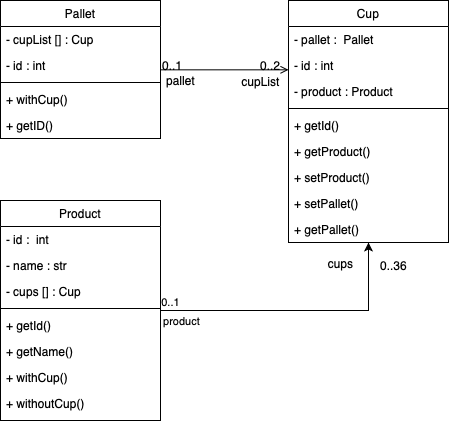
\includegraphics[width = \textwidth ]{Bilder/BeispielRefInt}
        \centering
\end{figure}

\newpage
\section{PySide6 und QuickQml 2.0}

Laut der Qt Wiki Website \cite{QtWikiHistory} wurde das Qt Framework geboren als ihre Schöpfer Haavard Nord und
Eric Chambe-Eng im Sommer 1990 in Norwegen an einem GUI für eine Ultraschall Datenbank arbeiten.
Die Software sollte damals in C++ implementiert auf Mac, Unix und Windows laufen.
Fünf Jahre später veröffentlichten Sie das erste Qt Framework unter dem Firmennamen Troll Tech.
Seitdem gewann das Framework immer mehr Popularität.
Im Jahr 2006 übernahm Nokia die Firma Trolltech und verkaufte das Qt Project in den Jahren 2011 und 2012 erst teilweise,
dann vollständig an den Digia Konzern.
Seit 2014 ist Qt als Tochterunternehmen des Digia Konzerns unter dem Namen \glqq The Qt Company\grqq ein eigenständiges Unternehmen.

Das Qt Framework ist in C++ implementiert und profitiert dadurch von dem Performance-Vorteil gegenüber anderen
Programmiersprachen.
Die neue Software für die $\mu$Plant soll jedoch in Python implementiert werden.
Für diese Zwecke hat Qt u.A. das Framework PySide6 veröffentlicht, welches einen Wrapper für Python Projekte bietet.

GUI's können in PySide6 im Wesentlichen auf zwei Arten erstellt werden.
Eine Möglichkeit ist es, das GUI über Widgets\cite{pysideQtWidgets} zu erstellen, die direkt im Python Code implementiert werden können.
Die zweite Möglichkeit ist QtQuick \cite{pysideQtQuick} zu nutzen, bei dem das GUI in einer separaten QML Datei erstellt wird und
mittels einer \verb|QtQmlApplicationEngine| Klasse in das Programm eingebunden wird.

Für die Umsetzung eines MVC-Design Patterns empfiehlt sich die Verwendung von QtQuickQML.
Durch die Verwendung des Frameworks wird die konsequente Trennung zwischen Interface und Datenmodell erzwungen.
Veranschaulicht wird dies in Abb. \ref{fig:figure10}.
Die eigentlichen Daten (von Server oder Datei) werden in ein Model überführt.
Dieses Model ist ein beliebig komplexes Klassenkonstrukt welches referenzielle Integrität aufbaut: Wird eine Stelle
berechtigter Weise geändert, bleibt das Modell intakt und im Sinne seiner Logik.
In Pyside6 muss dieses Datenmodell von der Basisklasse \verb|QAbstractModel| abgeleitet werden.
Beim Initialisierung der Anwendung wird eine Instanz dieser Klasse (oder einer abgeleiteten Klasse) erstellt und als
rootcontext der \verb|QQmlApplicationEngine| registriert.
Somit ist das Datenmodell mit dem GUI verknüpft und kann unter seiner URI in jedem QML File angesprochen werden.
In einer QML Datei wird ein entsprechendes QML Item, z.B. \verb|ListView|, welches eine einfache Liste erzeugt,
und dem Property \verb|model| die URI des Datenmodells zugewiesen.
Dadurch kennt das \verb|ListView| Objekt die Indices des Datenmodells und erhält beim rendern der Liste nur die benötigten
Teile der Daten.
Jede weitere Aktion die durch den Benutzer auf ein Listenelement ausgelöst wird, bezieht sich auf ein Delegate des Datenmodells.
Jede Änderung an dem Delegate wird zunächst gerendert und überprüft bevor das Datenmodell geändert wird.
Diese Basisfunktion kommt mit dem Qt Framework an sich und müssen nicht implementiert werden.
Wie jedoch das Datenmodell mit den geänderten Daten umgeht oder ob die Änderung des Datenmodells automatisch ein Update
der Daten auf dem Server oder der Datei auslöst, muss vom Entwickler implementiert werden!
An ein Delegate sind je nach QmlType durch das Framework Signale gebunden.
Signale sind Teil des Signal/Slot Prinzips des Qt Framework \cite{pysideSignalSlot} und stellen die Funktion eines Events dar.
Durch die \verb|QmlApplicationEngine| sind innerhalb eines GUIs alle rootContext Elemente ansprechbar.
Wird ein Signal an beliebiger Stelle im GUI emittiert, kann es an jeder anderen Stelle als Event genutzt werden.
Dadurch muss man  in der Regel keine zusätzlichen Callbacks oder Lamda-Ausdrücke definieren.
Außerhalb des QML Contexts, z.B. in einer Python Klasse, muss das Signal der Klasse bekannt sein, indem das Signal an die Klasse
gebunden wird.
Eine Funktion die mit der Annotation \glqq Slot(str) \grqq versehen ist, wird als Slot behandelt und kann mit dem Signal
verknüpft werden, sodass diese bei Auftreten des Signals ausgeführt werden.
Signale können Daten übergeben werden, die so an einen Slot übergeben werden können.\\
\vspace{1cm}
In meiner Vorbereitung auf diese Arbeit hat sich eine intuitive Vorgehensweise entwickelt, die ich für die Implementierung
der Software empfehlen möchte:\\
\vspace{1cm}
Beim initialisieren des Programms werden von allen Datenmodellen (\verb|QAbstractModel| und abgeleitete Klassen), Controllern
und Serviceklassen Instanzen erzeugt und als rootContext der \verb|QQmlApllicationEngine| gesetzt.
\lstset{
    basicstyle=\small\ttfamily
}
\lstinputlisting[language=Python]{Listings/Demo1.py}\label{exampleApp}
\begin{figure}
        \caption[Model-View Konzept mit zusätzlichem Controller und Service ]
        {\small Die Abbildung zeigt das in PySide6 verwendete Model-View Konzept, welches um einer Controllerklasse und
        einer Service Klasse erweitert wurde. }\label{fig:figure10}
        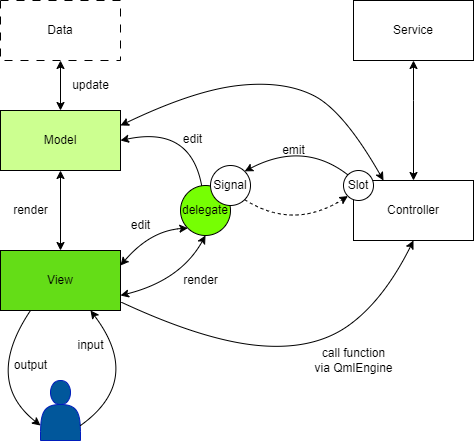
\includegraphics[width = \textwidth ]{Bilder/MVCS_Beispiel}
        \centering
\end{figure}

\section{GUI - Konzeptionierung}

\section{Konzepte zur Datenmodellierung}

\section{Konzepte für Controller- und Serviceklassen}

\section{Teilautomatisierte Code Dokumentation}